\section{Αριθμητικές Μαγνητοϋδροδυναμικές εξομοιώσεις}
Για να μελετήσουμε τη δυναμική των μοριακών νεφών στους γαλαξίες και τις αλληλεπιδράσεις τους με βίαια - ενεργητικά φαινόμενα όπως πίδακες από κέντρα γαλαξιών και αστρικούς ανέμους θα καταφύγουμε στην προσομοίωση τους μέσω της αριθμητικής επίλυσης των εξισώσεων της υδροδυναμικής και μαγνητουδροδυναμικής.

Ο υπολογιστικός κώδικας που θα χρησιμοποιήσουμε ονομάζεται PLUTO \cite{mignone_pluto:_2007} και παρακάτω θα εκθέσουμε σε γενικές γραμμές και όχι πολλές τεχνικές λεπτομέρειες το τρόπο με τον οποίο ο PLUTO αλλά και μια μεγάλη οικογένεια αντίστοιχων ολοκληρωτών επιλύουν τις αντίστοιχες εξισώσεις.

\subsection{Εξισώσεις Διατήρησης}
Οι εξισώσεις διατήρησης είναι χρονοεξαρτώμενα συστήματα μερικών διαφορικών εξισώσεων που έχουν τη γενική μορφή:
\begin{equation}
\label{eq:hyperbolicconservation}
\pdv{t} \bar{q}(x,t) + \pdv{x} \bar{f}(\bar{q}(x,t)) = 0 
\end{equation}
με $\bar{q}(x,t) \in \mathbb{R}^m$ ένα m-διάστατο άνυσμα των διατηρουμένων ποσοτήτων με  $\int_{-\infty}^{\infty} q_j (x,t) dx$ να είναι η ολική ποσότητα η οποία παραμένει σταθερή στο χρόνο t. 

Η $q_j(x,t)$ είναι ουσιαστικά η χωρική κατανομή (πυκνότητα) στο χρόνο $t$ η οποία γενικά μεταβάλλεται με το χρόνο.
Αυτή η μεταβολή περιγράφεται από τη συνάρτηση ροής $f_j(q(x,t))$. 
 
Το σύστημα \ref{eq:hyperbolicconservation} είναι η γενικότερη (μη γραμμική) μορφή των γραμμικών υπερβολικών εξισώσεων της μορφής:
\begin{equation}
\label{eq:linearhyperbolic}
\pdv{q}{t} +  \mathbf{A}\pdv{q}{x}  = 0 
\end{equation}
όπου $\mathbf{A}$ ένας τετραγωνικός διαγωνοποιήσιμος πίνακας με πραγματικές ιδιοτιμές.

Όπως και για τη μονοδιάστατη \todo{Λαθος} περίπτωση 
\begin{equation}
\label{eq:simple_advection}
\pdv{q}{t} +  u\pdv{q}{x}  = 0 
\end{equation}
η οποία έχει σαν λύση τη κυματική λύση D'Alembert
\begin{equation}
q(x,t)=q(x-ut,0)
\end{equation}
η γενική εξίσωση \ref{eq:linearhyperbolic} επιδέχεται αντίστοιχες κυματικές λύσεις.

Στη μη-γραμμική περίπτωση \ref{eq:hyperbolicconservation} το σύστημα λέγεται υπερβολικό αν ο ιακωβιανός πίνακας $\mathbf{J}(q)$ με στοιχεία $(i,j)$ τα $\pdv{f_i}{g_j}$ είναι αντίστοιχα διαγωνοποιήσιμος με πραγματικές ιδιοτιμές.

Τότε μπορούμε να γράψουμε το σύστημα των μη-γραμμικών εξίσωσεων στη μορφή:
\begin{equation}
\pdv{\bar{q}}{t} + \mathbf{J}(\bar{q}) \pdv{\bar{q}}{x} = 0 
\end{equation}

\subsection{Εξισώσεις Euler}
Οι εξισώσεις euler είναι ένα σύστημα μη-γραμμικών υπερβολικών μερικών διαφορικών εξισώσεων που περιγράφουν ένα ρευστό χωρίς ιξώδες και θερμική αγωγιμότητα\marginpar{Τα φαινόμενα διάχυσης (θερμική αγωγιμότητα, μοριακή διάχυση, ιξώδες) δίνουν όρους διάχυσης στη συνάρτηση ροής η οποία τώρα είναι της μορφής $f(q,q_x)$. Αποτέλεσμα αυτού είναι στο δεξί μέλος των εξισώσεων να εμφανίζονται όροι $\pdv*[2]{q}{x}$ και από υπερβολικές να γίνονται παραβολικές. Η πλήρης μορφή των υδροδυναμικών εξισώσεων δίνεται από τις εξισώσεις Navier-Stokes}.   
\begin{align}
&\pdv{\rho}{t} + \div(\rho \vec{u})=0 \label{eq:MassHD} && 
\texttt{Διατήρηση Μάζας} \\
&\pdv{t}(\rho  \vec{u})+\div(\rho  \vec{u}  \vec{u} +P)=0 && 
\texttt{Διατήρηση Ορμής} \label{eq:MomentumHD} \\
&\pdv{E}{t}+\div((E+P)\vec{u})=0 \label{eq:EnergyHD} && 
\texttt{Διατήρηση Ενέργειας}
\end{align}
με $E=\frac{P}{\gamma -1} +\frac{1}{2}\rho u^2$ η ενέργεια για ένα πολυτροπικό αέριο και $P$ η πίεση.

Σύμφωνα με τα προηγούμενα μπορούμε να γράψουμε το σύστημα στη μορφή \ref{eq:hyperbolicconservation}:
\begin{equation}
\pdv{t} \bar{q}(\vec{x},t) + \div\mathbf{f}(\bar{q}(\vec{x},t)) = 0 
\end{equation}
όπου 
\begin{equation}
\bar{q}(\vec{x},t)=\mqty(\rho \\ 
						\rho  \vec{u} \\
						E)
						=
						\mqty(q_1 \\ 
							  q_2 \\
							  q_3)
\end{equation}
και
\begin{equation}
\mathbf{f}(\bar{q}) = \mqty(\rho \vec{u} \\ 
						\rho \vec{u}\vec{u} + P \\
						\vec{u}(E+P))
					= \mqty(q_2 \\ 
						\frac{q_2 ^2}{q_1} +P(\bar{q}) \\
						\frac{q_2}{q_1} (q_3+P(\bar{q})))
\end{equation}
όπου $P(\bar{q})$ η καταστατική εξίσωση.


\subsection{Πηγές}
Μέχρι τώρα έχουμε υποθέσει ότι όλες οι διατηρούμενες ποσότητες, "διατηρούνται". Σε πραγματικές συνθήκες όμως υπάρχουν πηγές που προσθέτουν ή αφαιρούν (καταβόθρες) από τις ποσότητες μας. Μερικά παραδείγματα είναι:
\begin{itemize}
	\item Χημικές διεργασίες, ιονισμός και επανασύνδεση που ανταλλάσσουν / δημιουργούν / καταστρέφουν μάζες μεταξύ στοιχείων (διατήρηση της μάζας για πολλαπλά ρευστά)
	\item Εξωτερικές δυνάμεις όπως η βαρύτητα που λειτουργούν σαν πηγές στις εξισώσεις ορμής και ενέργειας.
	\item Μεταφορά θερμότητας μέσω ακτινοβολίας που λειτουργεί σαν πηγή (θέρμανση) ή καταβόθρα (ψύξη)
\end{itemize}
Οι εξισώσεις μας τότε αποκτούν τη μη ομογενή μορφή:
\begin{equation}
\pdv{t} \mathbf{q}(\vec{x},t) + \div\mathbf{f}(\mathbf{q}(\vec{x},t)) = S(\mathbf{q}(\vec{x},t))
\end{equation}

%\begin{marginfigure}
%	\label{fig:sodleveque}
%	\centering
%	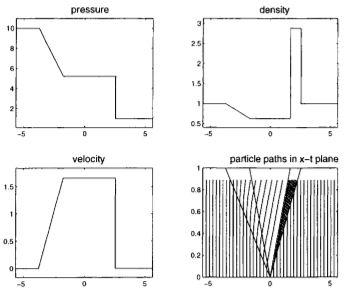
\includegraphics[width=1\linewidth]{Images/SODleveque}
%	\caption{Επίλυση του προβλήματος Riemann για τις μονοδιάστατες εξισώσεις Euler με αρχικές συνθήκες όπου η αρχική πίεση στα αριστερά είναι 10πλάσια της αρχικής πίεσης στα δεξιά ενώ οι αρχικές πυκνότητες μένουν ίδιες. Οι χαρακτηριστικές ταχύτητες είναι διαφορετικές (τελευταίο σχήμα) με αποτέλεσμα τα σωματίδια να πυκνώνουν και να δημιουργούν ένα κρουστικό κύμα πύκνωσης προς τα δεξιά, ενώ προς τα αριστερά δημιουργείται ένα κύμα αραίωσης. \cite{leveque_computational_1998}}
%\end{marginfigure}



\subsection{Αριθμητική επίλυση υπερβολικών εξισώσεων}
Η αριθμητική επίλυση των υπερβολικών εξίσωσεων αποτελεί μια δύσκολη διαδικασία
\subsubsection{Μέθοδος πεπερασμένων διαφορών}
Η βασική αρχή της μεθόδου των πεπερασμένων διαφορών -όπως και μεθόδων που πηγάζουν από αυτή και θα δούμε στη συνέχεια- είναι η διακριτοποιήση του χώρου και του χρόνου. Δηλαδή αναζητούμε μια προσεγγιστική τιμή των προς αναζήτηση ποσοτήτων σε συγκεκριμένα σημεία στο χώρο και στο χρόνο. Αν διακριτοποιήσουμε το χώρο κατα αποστάσεις $\Delta x=\Delta y = h$ και στο χρόνο $\Delta t=k$ τότε η προσεγγιστική τιμή στη θέση $(x_\mathrm{i},y_\mathrm{j})=(x_0+\mathrm{i}h,y_0+\mathrm{j}h)$ και στο χρόνο $t_\mathrm{n}=t_0+\mathrm{n}k$ θα είναι:
\begin{equation}
Q_{\mathrm{ij}}^\mathrm{n }\simeq q(x_\mathrm{i},y_\mathrm{j},t_\mathrm{n})
\end{equation}
Οπότε μια (για παράδειγμα μονοδιάτατη) μερική διαφορική εξίσωση της μορφής
\begin{equation}
\pdv{q}{t}+u\pdv{q}{x}=0
\end{equation} 
θα γράφεται:
\begin{equation}
\frac{Q_\mathrm{i}^\mathrm{n+1}-Q_\mathrm{i}^n }{k} + u \left( \frac{Q_\mathrm{i}^\mathrm{n+1}-Q_\mathrm{i}^\mathrm{n} }{k}  \right) =0
\end{equation}
άρα με βάση τις αρχικές συνθήκες $q_i^0$ μπορούμε να ολοκληρώσουμε στο χρόνο, άρα η λύση στο κελί με συντεταγμένες $\mathrm{ijn}$ θα είναι:
\begin{equation}
Q_{\mathrm{i}}^\mathrm{n+1} = Q_{\mathrm{i}}^\mathrm{n} -\frac{k}{h} u \left( Q_\mathrm{i}^\mathrm{n} - Q_\mathrm{i-1}^\mathrm{n} \right)
\end{equation} 

Αντίστοιχα στη περίπτωση ενός συστήματος εξισώσεων η λύση θα ήταν
\begin{equation}
Q_{\mathrm{i}}^\mathrm{n+1} = Q_{\mathrm{i}}^\mathrm{n} -\frac{k}{h} \mathbf{Α} \left( Q_\mathrm{i}^\mathrm{n} - Q_\mathrm{i-1}^\mathrm{n} \right)
\end{equation} 
με τον πίνακα $\mathbf{Α}$ να έχει θετικές ιδιοτιμές. 

Η τιμή των ποσοτήτων σε ένα κελί παρατηρούμε ότι εξαρτάται από τις τιμές των αμέσως γειτονικών κελιών. Η ακρίβεια μας τώρα είναι της τάξης του $h$ \todo{γιατί? Taylor}. Για να πετύχουμε μεγαλύτερη ακρίβεια μπορούμε να ανανεώνουμε τις ποσότητες $q_j$ με βάση πιο απομακρυσμένα κελιά, όπως για παράδειγμα η μέθοδος leapfrog:
\begin{equation}
Q_{\mathrm{i}}^\mathrm{n+1} = Q_{\mathrm{i}}^\mathrm{n-1} -\frac{k}{h} \mathbf{Α} \left( Q_\mathrm{i+1}^\mathrm{n} - Q_\mathrm{i-1}^\mathrm{n} \right)
\end{equation} 
ή να κρατήσουμε τους 3 πρώτους όρους από το αναπτύγμα Taylor $q(x,t+k)=q(x,t)+k\pdv{q}{t}(x,t)+\frac{1}{2}k^2 \pdv[2]{q}{t}$ τη μέθοδο Lax-Wendroff:
 
 \begin{equation}
 Q_{\mathrm{i}}^\mathrm{n+1} = Q_{\mathrm{i}}^\mathrm{n} -\frac{k}{2h} \mathbf{Α} \left( Q_\mathrm{i+1}^\mathrm{n} - Q_\mathrm{i-1}^\mathrm{n} \right) +\frac{k^2}{2h^2} \mathbf{Α}^2 \left( Q_\mathrm{i+1}^\mathrm{n} - 2Q_{\mathrm{i}}^\mathrm{n}+ Q_\mathrm{i-1}^\mathrm{n} \right)
 \end{equation} 
 
 Παρά το βαθμό ακρίβεια της κάθε μέθοδο μεταξύ των παραπάνω, οι μέθοδοι πεπερασμένων διαφορών δεν καταφέρνουν να διατηρήσουν τις ολοκληρώσιμες ποσότητες ειδικά όταν εμπλέκονται κρουστικά κύματα και ασυνέχειες. Γι αυτό το σκοπό θα χρησιμοποιήσουμε τις λεγόμενες μεθόδους πεπερασμένων όγκων.
 
\subsubsection{Μέθοδος Πεπερασμένων Όγκων}
Αντί για τη προσεγγιστική τιμή $Q_{\mathrm{i}}^\mathrm{n+1}$ της $q(x_\mathrm{i},t_\mathrm{n+1})$ σε ένα συγκεκριμένο σημείο θα ορίσουμε μια νέα αντίστοιχη τιμή για τη μέση τιμή της ποσότητας σε κάθε ένα διάστημα $C_\mathrm{i}=[x_\mathrm{i},x_\mathrm{i+1}]$ του χώρου μας με $x_\mathrm{i}=x_0+(i-1)h$. 

Άρα τώρα η τιμή $Q_{\mathrm{i}}^\mathrm{n}$ θα προσεγγίζει την μέση τιμή στο $\mathrm{i}$ διάστημα τη χρονική στιγμή $t_\mathrm{n}$
\begin{equation}
Q_{\mathrm{i}}^\mathrm{n} \simeq \frac{1}{h} \int _{C_\mathrm{i}} q(x,t_\mathrm{n})dx
\end{equation}
Αν η $q(x,t)$ δεν περιέχει ασυνέχειες τότε η $Q_{\mathrm{i}}^\mathrm{n}$ τη προσεγγίζει στο μέσο του διαστήματος με ακρίβεια τάξης μεγέθους $\order{h^2}$.

Αν πάρουμε την ολοκληρωτική μορφή του νόμου διατήρησης σε ένα κελί η εξέλιξη στο χρόνο θα είναι
\begin{equation}
\int _{C_\mathrm{i}} q(x,t_\mathrm{n+1})dx -\int _{C_\mathrm{i}} q(x,t_\mathrm{n})dx = 
\int_{t_\mathrm{n}}^{t_\mathrm{n+1}} f(q(x_\mathrm{i},t))dt - \int_{t_\mathrm{n}}^{t_\mathrm{n+1}} f(q(x_\mathrm{i+1},t))dt
\end{equation}

\marginpar{
Αν αναδιατάξουμε τη σχέση \ref{eq:FVM} κατάλληλα βρίσκουμε:
\begin{equation}
\frac{Q_{\mathrm{i}}^\mathrm{n+1} - Q_{\mathrm{i}}^\mathrm{n}}{k} +\frac{F_{\mathrm{i+1}}^\mathrm{n} - F_{\mathrm{i}}^\mathrm{n}}{h}=0
\end{equation}
η οποία είναι η εξίσωση του νόμου διατήρησης. Ακρι
}
\begin{marginfigure}
	\centering
	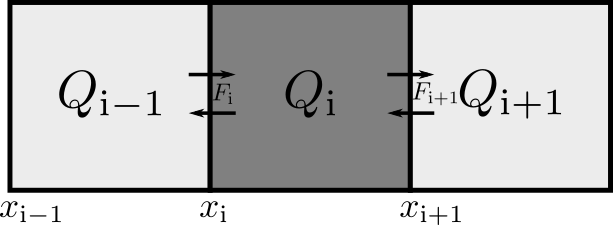
\includegraphics[width=1\linewidth]{Images/FVM}
	\caption{}
	\label{fig:fvm}
\end{marginfigure}


διαιρώντας με $h$ και αντικαθιστώντας τις $Q_{\mathrm{i}}^\mathrm{n}$ βρίσκουμε την εξέλιξη στο χρόνο
\begin{equation}
Q_{\mathrm{i}}^\mathrm{n+1} = Q_{\mathrm{i}}^\mathrm{n} - \frac{1}{h}\left( \int_{t_\mathrm{n}}^{t_\mathrm{n+1}} f(q(x_\mathrm{i},t))dt - \int_{t_\mathrm{n}}^{t_\mathrm{n+1}} f(q(x_\mathrm{i+1},t))dt \right) 
\end{equation}
και τελικά
\begin{equation}
\label{eq:FVM}
Q_{\mathrm{i}}^\mathrm{n+1} = Q_{\mathrm{i}}^\mathrm{n} - \frac{k}{h}\left(F_{\mathrm{i+1}}^\mathrm{n}-F_{\mathrm{i}}^\mathrm{n} \right) 
\end{equation}
όπου 
\begin{equation}
F_{\mathrm{i}}^\mathrm{n} \simeq \frac{1}{k}\int_{t_\mathrm{n}}^{t_\mathrm{n}}f(q(x_\mathrm{i},t))dt 
\end{equation}
η προσεγγιστική τιμή της μέσης ροής κατά μήκος της $x_\mathrm{i}$. Είναι λογικό να υποθέσουμε ότι η ροή στο σύνορο μεταξύ δύο κελιών εξαρτάται από τις τιμές των ποσοτήτων σε αυτά τα δύο κελιά, δηλαδή %η συνάρτηση της ροής
\begin{equation}
F_{\mathrm{i}}^\mathrm{n} = F\left( Q_{\mathrm{i-1}}^\mathrm{n} ,Q_{\mathrm{i}}^\mathrm{n} \right) 
\end{equation}
άρα αν γνωρίζουμε αυτή τη συνάρτηση ροής τότε μπορούμε να υπολογίσουμε την εξέλιξη στο χρόνο της μέσης τιμής του κάθε κελιού
\begin{equation}
Q_{\mathrm{i}}^\mathrm{n+1} = Q_{\mathrm{i}}^\mathrm{n} - \frac{k}{h}\left(
F\left( Q_{\mathrm{i}}^\mathrm{n} ,Q_{\mathrm{i+1}}^\mathrm{n} \right)-
F\left( Q_{\mathrm{i-1}}^\mathrm{n} ,Q_{\mathrm{i}}^\mathrm{n} \right)
 \right) 
\end{equation} 

Η μέθοδος (ή καλύτερα η οικογένεια μεθόδων) που ακολουθούμε στην εύρεση των συναρτήσεων ροής ονομάζεται μέθοδος Godunov, από τον Sergei K. Godunov που πρώτος την εισήγαγε το 1959. Η μέθοδος αυτή βασίζεται στην επίλυση του προβλήματος Riemann μεταξύ των κελιών.
Παρακάτω θα αναπτύξουμε το πως λύνεται το πρόβλημα Riemann.
 

\subsection{Πρόβλημα Riemann}
Το πρόβλημα Riemann είναι η επίλυση του νόμου διατήρησης της μορφής
\begin{equation}
\pdv{\bar{q}}{t}+\pdv{f(\bar{q})}{x}=0
\end{equation}
με αρχικές συνθήκες όπου υπάρχει μια ασυνέχεια:
\begin{equation}
\bar{q}(x,0)=
\begin{cases}
\bar{q}_\mathrm{L} &\qq{για} x<0 \\
\bar{q}_\mathrm{R} &\qq{για} x>0 
\end{cases}
\end{equation}

%Όπως βλέπουμε χαρακτηριστικά και στο shock tube problem (\ref{fig:sodleveque}), λόγω της αρχικής ασυνέχειας και της μη-γραμμικότητας των εξισώσεων euler έχουμε σαν αποτέλεσμα τη δημιουργία κρουστικών κυμάτων.
Για να δώσουμε μια αναλυτική λύση στο γενικό πρόβλημα (μη-γραμμικό) Riemann θα ξεκινήσουμε από τη γραμμική περίπτωση.

\subsubsection{Γενική επίλυση του γραμμικού προβλήματος Riemann}
Η επίλυση του προβλήματος Riemann στη γραμμική περίπτωση του νόμου διατήρησης, δηλαδή στο σύστημα
\begin{equation}
\pdv{\bar{q}}{t} +  \mathbf{A}\pdv{\bar{q}}{x}  = 0 
\end{equation}
 βασίζεται στο μετασχηματισμό των ποσοτήτων $\bar{q}$ στις λεγόμενες χαρακτηριστικές μεταβλητές $\bar{\xi}=\mathbf{R}^{-1}\bar{q}$ όπου $\mathbf{R}=(\bar{r}_1,\bar{r}_2,\cdots \bar{r}_m)$ είναι ο πίνακας των ιδιοανυσμάτων του πίνακα $\mathbf{A}$, ενώ με $\bar{\Lambda}=\mathtt{diag}(\lambda _1,\lambda _2,\cdots \lambda _m)$ ορίζουμε το διαγώνιο πίνακα των ιδιοτιμών. Για τον πίνακα $\mathbf{A}$ ισχύει\ ότι $\mathbf{A}=\mathbf{R}\bar{\Lambda}\mathbf{R}^{-1}$.

Οι εξισώσεις τότε γράφονται:
\begin{equation}
\pdv{\bar{\xi}}{t} + \bar{\Lambda} \div\bar{\xi} =0
\end{equation} 
δηλαδή σαν ένα διαχωρισμένο σύστημα εξισώσεων της μορφής 
\begin{equation}
\pdv{q}{t} +  u\pdv{q}{x}  = 0 
\end{equation} που όπως έχουμε δει ήδη έχουν λύσεις:
\begin{equation}
\label{eq:xi_solution}
\xi_p  = \xi_p(x-\lambda _p t,0) 
\end{equation}
με $p=1...m$ για τις $m$ εξισώσεις (μονοδιάστατη περίπτωση). Οι $p$ χαρακτηριστικές καμπύλες δηλαδή καθορίζονται από τις ιδιοτιμές $\lambda _p$.

Άρα αν επιστρέψουμε στις αρχικές μεταβλητές:
\begin{equation}
\bar{q}(x,t) = \sum_{p=1}^{m} \xi_p(x-\lambda _p t,0)\bar{r}_p
\end{equation}

\begin{marginfigure}
	\centering
	\label{fig:linearriemann-leveque}
	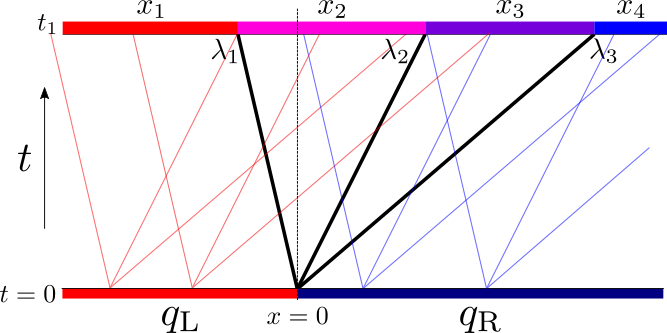
\includegraphics[width=1\linewidth]{Images/reimannlinear.png}
	\caption{Γραφική απεικόνιση της λύση του γραμμικού προβλήματος Riemann για $p=3$. 
		Τη χρονική στιγμή $t_1$ οι λύσεις σε κάθε σημείο του χώρου καθορίζονται απόλυτα από τις $p$ χαρακτηριστικές ιδιοτιμές $\lambda _p$ έτσι ώστε η τελική λύση για κάθε σημείο $x$ να είναι ο γραμμικός συνδυασμός των περιοχών που επηρεάζουν αυτό το σημείο, δηλαδή}	
	\begin{align*}
	q(x_1,t_1)&=\xi _1 ^L r_1 +\xi _2 ^L r_2 + \xi _3 ^L r_3 \\
	q(x_2,t_1)&=\xi _1 ^R r_1 +\xi _2 ^L r_2 + \xi _3 ^L r_3 \\
	q(x_3,t_1)&=\xi _1 ^R r_1 +\xi _2 ^R r_2 + \xi _3 ^L r_3 \\
	q(x_4,t_1)&=\xi _1 ^R r_1 +\xi _2 ^R r_2 + \xi _3 ^R r_3 
	\end{align*} 
	
\end{marginfigure}
Για τις αρχικές συνθήκες του προβλήματος Riemann o μετασχηματισμός μας δίνει:
\begin{equation}
\xi_p (x,0) =
\begin{cases}
\xi^\mathrm{L}_p &\qq{για} x<0 \\
\xi^\mathrm{R}_p &\qq{για} x>0 
\end{cases}
\end{equation} 

άρα από \ref{eq:xi_solution}
\begin{equation}
\xi_p (x,t) =
\begin{cases}
\xi^\mathrm{L}_p &\qq{για} x-\lambda _p t<0 \\
\xi^\mathrm{R}_p &\qq{για} x-\lambda _p t>0 
\end{cases}
\end{equation} 




Άρα με αρχικές συνθήκες Riemann, βλέπουμε ότι η λύση για τις μετασχηματισμένη μεταβλητή $\xi _p$ σε ένα οποιαδήποτε σημείο εξαρτάται απόλυτα αό τη σχετική θέση σε σχέση με την αντίστοιχη χαρακτηριστική καμπύλη της $\lambda _p$.  

Καθώς διασχίζουμε τη καμπύλη αυτή ουσιαστικά μετακινούμαστε από τις συνθήκες $\xi^L_p$ στις $\xi^R_p$. Το άλμα αυτό υπακούει τις συνθήκες Rankine-Hugoniot \todo{Rankine-Hugoniot} άρα για κάθε σημείο μπορούμε τελικά να γράψουμε τη λύση.
\begin{equation}
\bar{q}(x,t)=q_L + \sum_{\lambda_p<x/t} (\xi ^R_P - \xi ^L_P) \bar{r_p}
			=q_R - \sum_{\lambda_p>x/t} (\xi ^R_P - \xi ^L_P) \bar{r_p}
\end{equation}
\todo{Επιλυση γραμμικου Riemann διαγραμμα}

\subsubsection{Επίλυση του μη γραμμικού προβλήματος Riemann}
Στη μη γραμμική περίπτωσή των νόμων διατήρησης, όπως είναι και οι εξισώσεις Euler, η συνάρτηση ροής της διατηρούμενης ποσότητας εξαρτάται πια από την ίδια τη ποσότητα, δηλαδή:
\begin{equation}
\pdv{t} \bar{q}(x,t) + \pdv{x} \bar{f}(\bar{q}(x,t)) = 0 
\end{equation}

Για ομαλές λύσεις μπορούμε να μετασχηματίσουμε το παραπάνω σύστημα μέσω της ιακωβιανής $\mathbf{J} =\mathbf{f}'$
\begin{equation}
\pdv{t} \bar{q}(x,t) + \mathbf{J}(q(x,t)) \pdv{q}{x}  = 0 
\end{equation}

Λειτουργώντας όπως και στη γραμμική περίπτωση παρατηρούμε ότι οι ιδιοτιμές και τα ιδιοανύσματα της ιακωβιανής είναι συναρτήσεις των ποσοτήτων $q_\mathrm{j}$. Δηλαδή οι κλίσεις των χαρακτηριστικών καμπύλων μπορούν να αλλάζουν κλίση στο χώρο και στο χρόνο. 

Συμπεραίνουμε λοιπόν ότι σε περιοχές ανάμεσα σε αυτές οι λύσεις περιγράφονται ακριβώς όπως και στη γραμμική περίπτωση, ενώ ταυτόχρονα έχουμε και τη δημιουργία 2 νέων "χαρακτηριστικών" καμπυλών - κυμάτων στα σημεία μεταξύ αυτών των περιοχών.

Στις περιοχές όπου οι χαρακτηριστικές καμπύλες συγκλίνουν έχουμε τα λεγόμενα κρουστικά κύματα τα οποία διαδίδονται με ταχύτητα \todo{shock wave speed} και στις περιοχές που αποκλίνουν τα κύματα αραίωσης.

Άρα για να υπολογίσουμε 

\begin{marginfigure}
	\centering
	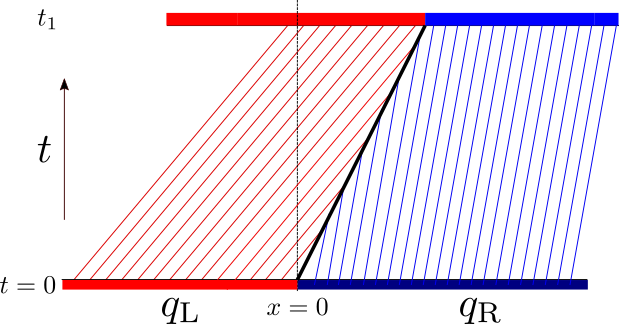
\includegraphics[width=1\linewidth]{Images/shockwave}
	\caption{}
	\label{fig:shockwave}
\end{marginfigure}


\begin{marginfigure}
	\centering
	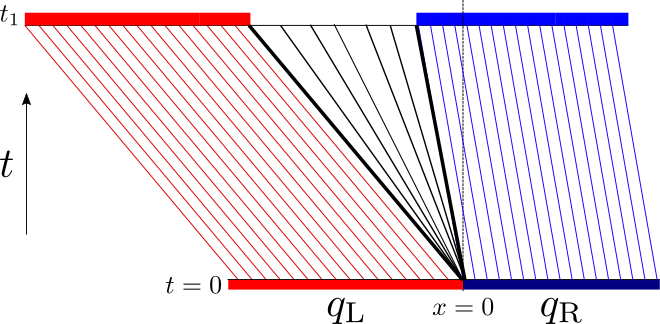
\includegraphics[width=1\linewidth]{Images/rarefuctionwave}
	\caption{}
	\label{fig:rarefuctionwave}
\end{marginfigure}



\subsection{Κώδικας PLUTO}

